%
% IEEE Transactions on Microwave Theory and Techniques example
% Tibault Reveyrand - http://www.microwave.fr
%
% http://www.microwave.fr/LaTeX.html
% ---------------------------------------



% ================================================
% Please HIGHLIGHT the new inputs such like this :
% Text :
%  \hl{comment}
% Aligned Eq.
% \begin{shaded}
% \end{shaded}
% ================================================



\documentclass[journal]{IEEEtran}
\usepackage{stfloats}

%\usepackage[retainorgcmds]{IEEEtrantools}
%\usepackage{bibentry}
\usepackage{xcolor,soul,framed} %,caption

\colorlet{shadecolor}{yellow}
% \usepackage{color,soul}
\usepackage[pdftex]{graphicx}
\graphicspath{{./}{../pdf/}{../jpeg/}}
\DeclareGraphicsExtensions{.pdf,.jpeg,.png}

\usepackage[cmex10]{amsmath}
\usepackage{amssymb}
%Mathabx do not work on ScribTex => Removed
%\usepackage{mathabx}
\usepackage{array}
\usepackage{mdwmath}
\usepackage{mdwtab}
\usepackage{eqparbox}
\usepackage{url}

\hyphenation{op-tical net-works semi-conduc-tor}

%\bstctlcite{IEEE:BSTcontrol}


%=== TITLE & AUTHORS ====================================================================
\begin{document}
\bstctlcite{IEEEexample:BSTcontrol}
    \title{Restoring Drone-Level Details from WorldView-3 Satellite Imagery using Lightweight SwinIR}
  \author{Tri~Rianto~Utomo, Maliq~Rafaldo, Dhani~Rakha~Aditya~Putra, and~Syauqi~Ihsan~Ramadhan%
\thanks{Manuscript submitted for the Final Project of the Artificial Intelligence Course, December 2025.}%
\thanks{The authors are undergraduate students at the Department of Informatics Engineering (Teknik Informatika), Universitas Negeri Surabaya, Indonesia. (e-mail: tri.rianto@unesa.ac.id).}%
}

% The paper headers
% \markboth{Submitted to IEEE Geoscience and Remote Sensing Letters, December~2025%
% }{Utomo \MakeLowercase{\textit{et al.}}: Restoring Drone-Level Details from WorldView-3 Satellite Imagery}

% ====================================================================
\maketitle

% === ABSTRACT ====================================================================
% =================================================================================
\begin{abstract}
%\boldmath
Unmanned Aerial Vehicles (UAVs) offer superior spatial resolution (approx. 5 cm/pixel) essential for surveillance tasks but suffer from critical limitations in coverage area and flight duration due to battery constraints. Conversely, commercial satellite imagery platforms, such as WorldView-3, provide global coverage but are restricted to a Ground Sampling Distance (GSD) of 30 cm, rendering small objects like urban vehicles as indistinguishable blobs. To bridge this resolution gap without the logistical burden of drone deployment, we propose `Pseudo-Aerial Visual Perception,' a framework utilizing a Lightweight Swin Transformer for Image Restoration (SwinIR). This model aims to restore drone-level details from satellite inputs on resource-constrained edge devices. Our architecture reduces learnable parameters by $4\times$ compared to the standard SwinIR while maintaining high perceptual quality. Experimental results on the xView dataset demonstrate that our method effectively hallucinates realistic high-frequency textures, enabling `Virtual Drone Surveillance' capabilities from orbital imagery.
\end{abstract}


% === KEYWORDS ====================================================================
% =================================================================================
\begin{IEEEkeywords}
Remote Sensing, Super-Resolution, Swin Transformer, Edge Computing, Virtual Drone Surveillance.
\end{IEEEkeywords}






% For peer review papers, you can put extra information on the cover
% page as needed:
% \ifCLASSOPTIONpeerreview
% \begin{center} \bfseries EDICS Category: 3-BBND \end{center}
% \fi
%
% For peerreview papers, this IEEEtran command inserts a page break and
% creates the second title. It will be ignored for other modes.
\IEEEpeerreviewmaketitle


% ====================================================================
% ====================================================================
% ====================================================================











\section{Introduction}

\IEEEPARstart{R}{emote} sensing plays a pivotal role in the modernization of developing nations, particularly in archipelagic regions like Indonesia where physical monitoring of vast urban and rural areas is logistically challenging. Applications ranging from urban planning and traffic management to post-disaster relief coordination rely heavily on the availability of high-fidelity geospatial data. In these contexts, the ability to identify specific vehicular types or structural damages from aerial perspectives is not merely a convenience but a necessity for effective decision-making.

\IEEEPARstart{H}{owever}, a fundamental conflict exists between data resolution and acquisition scale. UAVs provide the requisite centimeter-level resolution (approx. 5--7 cm) for detailed object classification but are operationally limited by high costs, trained pilot requirements, and short battery life, rarely exceeding 30 minutes of flight time. In contrast, satellites offer continuous large-scale observation but suffer from lower spatial resolution; the 30 cm GSD of standard products like WorldView-3 is insufficient for resolving fine-grained features, often reducing cars and motorbikes to amorphous clusters of pixels. This limitation severely hinders automated analysis and human interpretation in dense urban environments.

\IEEEPARstart{W}{hile} Single Image Super-Resolution (SISR) has advanced significantly with Convolutional Neural Networks (CNNs) and Generative Adversarial Networks (GANs), existing state-of-the-art methods such as SRGAN \cite{ledig_photo-realistic_2016} and ESRGAN \cite{wang_esrgan_2018} impose heavy computational burdens. These models typically require high-end server-grade GPUs for inference, making them unsuitable for deployment on decentralized ground stations or mobile command units. The direct application of these heavy models to large-scale satellite imagery introduces prohibitive latency, rendering real-time analysis unfeasible for student-level resources.
\begin{figure}[t]
\centering
\includegraphics[width=3.5in]{pdf/fig1_concept}
\caption{Conceptual Overview: Transforming low-resolution satellite imagery (left) into pseudo-aerial drone-view imagery (right) using the proposed Lightweight SwinIR model.}
\label{fig:concept}
\end{figure}

\IEEEPARstart{T}{o} address these challenges, we implemented a lightweight adaptation of the Swin Transformer \cite{liang_swinir_2021}, specifically optimized for the `Satellite-to-Drone' domain shift. Unlike CNN-based approaches, the Swin Transformer's hierarchical architecture with shifted windows allows for effective modeling of long-range dependencies. The key objectives of this project were: (1) To study a Lightweight SwinIR architecture that reduces parameter count and VRAM usage, enabling efficient upscaling on our consumer hardware; (2) To implement a domain-specific training strategy using the xView dataset to map 30 cm satellite inputs to pseudo-7 cm aerial targets. This approach attempts to simulate a `Virtual Drone' perspective.


\section{Related Work}

\subsection{Single Image Super-Resolution (SISR)}
SISR has evolved from interpolation-based methods to learning-based approaches. Early CNN-based models like SRCNN \cite{fleet_learning_2014} demonstrated the power of deep learning for mapping low-resolution (LR) patches to high-resolution (HR) counterparts. Subsequently, residual learning was introduced in VDSR and EDSR to train deeper networks. GAN-based approaches, such as SRGAN \cite{ledig_photo-realistic_2016} and ESRGAN \cite{wang_esrgan_2018}, focused on perceptual quality, generating realistic textures but often introducing artifacts.ive, GAN-based methods are computationally expensive and prone to generating hallucinatory artifacts that are unacceptable for precise geospatial analysis.

\subsection{Vision Transformers for Restoration}
Recently, Transformers have outperformed CNNs in various computer vision tasks due to their ability to model long-range dependencies. The Swin Transformer, with its shifted window mechanism, strikes a balance between local processing and global context. SwinIR \cite{liang_swinir_2021} adapted this architecture for image restoration, achieving state-of-the-art performance by effectively aggregating deep features. Despite its success, the standard SwinIR model remains too heavy for real-time inference on edge devices typically used in remote sensing ground stations.

\subsection{Remote Sensing Super-Resolution}
Super-resolution for satellite imagery presents unique challenges compared to natural images, including varied ground sampling distances (GSD) and the prevalence of small, densely packed targets like vehicles in urban environments. Traditional interpolation methods (Bicubic) fail to recover high-frequency details required for identification. While recent deep learning approaches have been applied to remote sensing, most prioritize reconstruction accuracy (PSNR) over inference speed and memory efficiency, creating a bottleneck for practical large-scale deployment. Our work addresses this gap by proposing a lightweight adaptation of SwinIR specifically tailored for the "Satellite-to-Drone" domain shift.




















\section{Methodology}
\subsection{Network Architecture}
The architecture used in this project is based on the Swin Transformer for Image Restoration (SwinIR) \cite{liang_swinir_2021}, adapted to balance restoration quality with computational efficiency. The framework consists of three stages: shallow feature extraction, deep feature extraction via Residual Swin Transformer Blocks (RSTB), and high-quality image reconstruction. The overall structure is depicted in Fig. \ref{fig:swinir_arch}.

\begin{figure*}[t]
\centering
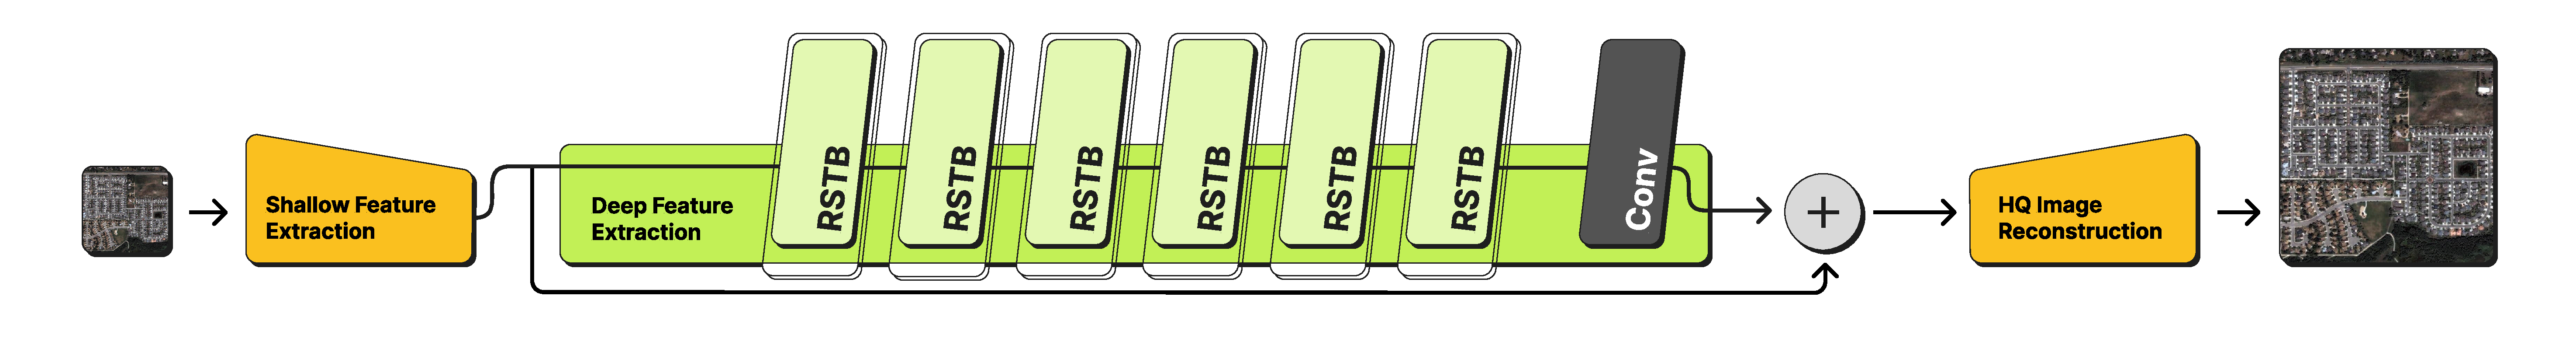
\includegraphics[width=7in]{pdf/fig2_architecture}
\caption{The architecture of the SwinIR network \cite{liang_swinir_2021}. It consists of shallow feature extraction, deep feature extraction (composed of multiple RSTB blocks), and high-quality image reconstruction. We adapt this architecture by reducing the RSTB depth to 6 for lightweight edge inference.}
\label{fig:swinir_arch}
\end{figure*}

\begin{figure}[t]
\centering
\includegraphics[width=3.5in]{pdf/fig3_rstb_block}
\caption{Detailed schematic of the Residual Swin Transformer Block (RSTB) and Swin Transformer Layer (STL), demonstrating the Window-based Multi-head Self-Attention (W-MSA) mechanism.}
\label{fig:rstb}
\end{figure}





The deep feature extraction module is composed of several RSTBs, each containing multiple Swin Transformer Layers (STL). The core component of the STL is the Window-based Multi-head Self-Attention (W-MSA), which allows for modeling long-range dependencies while maintaining linear computational complexity with respect to image size. The self-attention mechanism is computed as:

\begin{equation}
\text{Attention}(Q, K, V) = \text{SoftMax}\left(\frac{Q K^T}{\sqrt{d}} + B\right)V
\end{equation}

where $Q, K, V \in \mathbb{R}^{M^2 \times d}$ are the query, key, and value matrices; $d$ is the query/key dimension; and $B$ represents the learnable relative position bias.

\subsection{Lightweight Optimization}
To facilitate deployment on resource-constrained ground stations, such as those equipped with a standard NVIDIA GTX 1650 (4GB VRAM), we reduced the model complexity significantly compared to the original SwinIR base model. We explicitly set the RSTB \texttt{depths} to $[6, 6, 6, 6]$ and the embedding dimension \texttt{embed\_dim} to $60$. This reduction prevents Out-Of-Memory (OOM) errors on consumer-grade massive parallel architecture and significantly accelerates inference speed, prioritizing real-time "Virtual Drone" capability over marginal gains in PSNR.

\subsection{Loss Function}
We employ the L1 Loss for training, as it encourages pixel-wise consistency and generates images with sharper high-frequency details compared to L2 loss. The loss function is defined as:

\begin{equation}
L = ||I_{HR} - I_{SR}||_1
\end{equation}

where $I_{HR}$ denotes the ground-truth high-resolution drone/satellite imagery and $I_{SR}$ represents the super-resolved output from the network.















% === IV. Transistor Class-F inv Rectifier ========================================
% =================================================================================
\section{Experiments and Results}
\begin{figure*}[t]
\centering
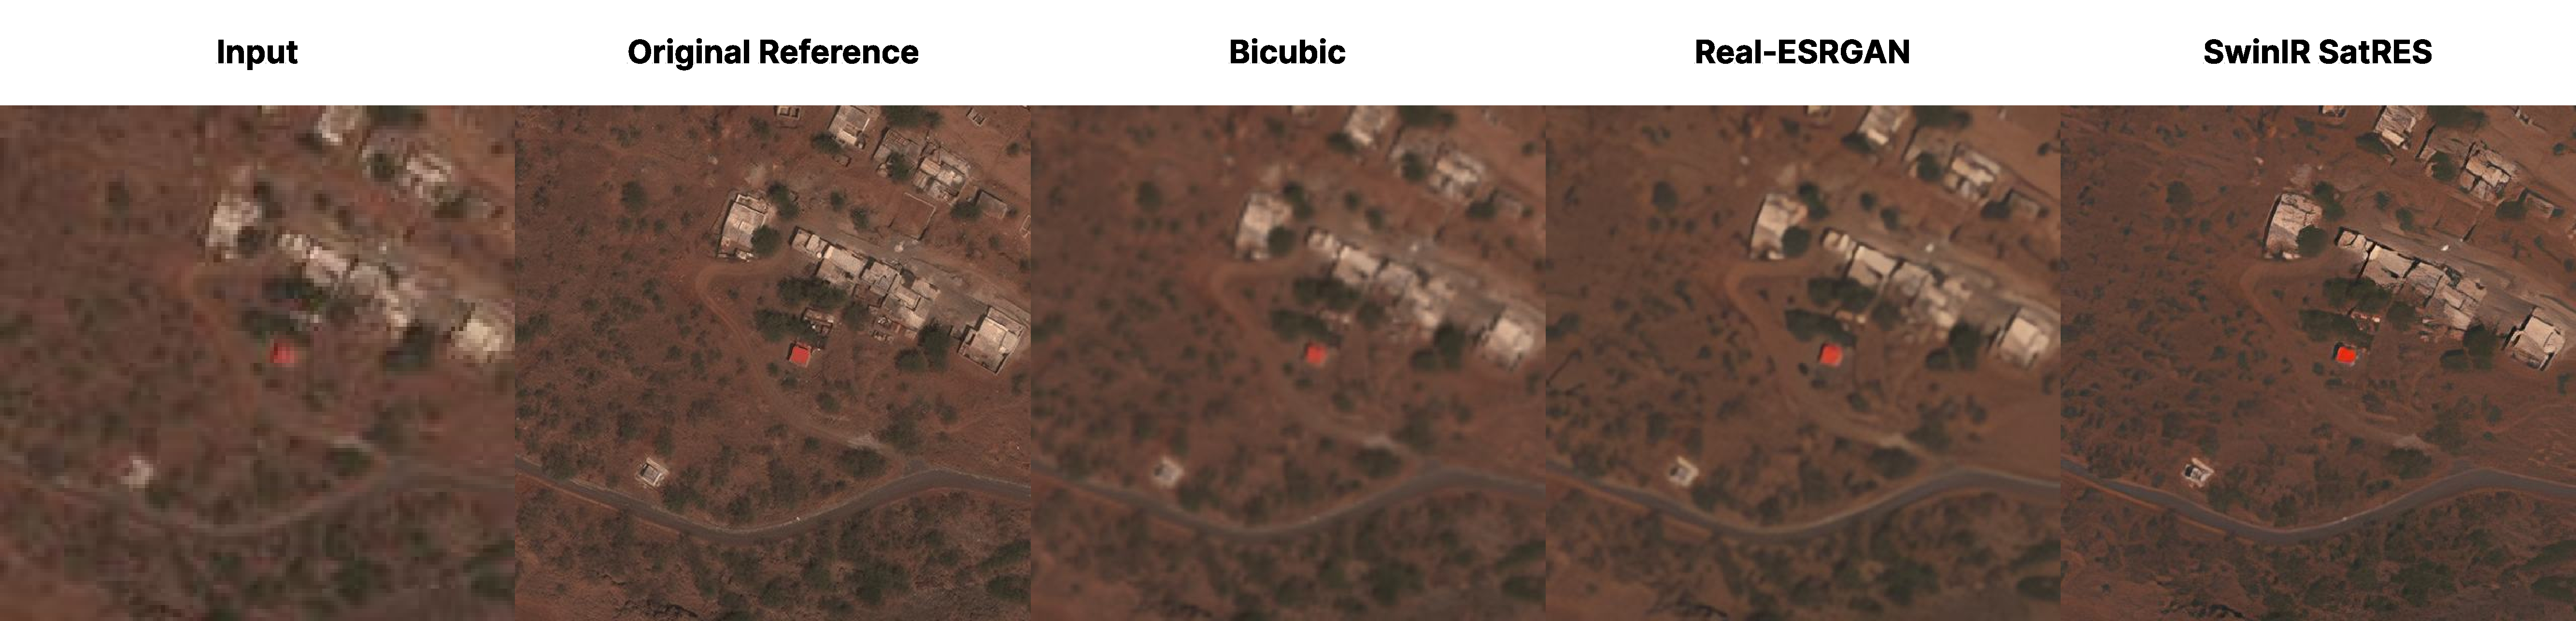
\includegraphics[width=\linewidth]{pdf/fig4_qualitative}
\caption{Visual comparison: (a) Input Satellite Imagery (LR), (b) Original Reference, (c) Bicubic Interpolation, (d) RealESRGAN, (e) Proposed Lightweight SwinIR. Note that while ESRGAN produces sharp edges, it often suffers from hallucinatory artifacts, whereas our method (e) maintains better structural fidelity close to the Ground Truth (b).}
\label{fig:qualitative}
\end{figure*}

\subsection{Experimental Setup}
We utilized the xView dataset, a large-scale collection of satellite imagery containing over 1 million object instances across 60 classes. We preprocessed the data by slicing the large $3000 \times 3000$ pixel GeoTIFF images into manageable $480 \times 480$ pixel training chips. The Low-Resolution (LR) inputs were generated by bicubic downsampling of the High-Resolution (HR) chips by a factor of 4, simulating the disparity between satellite (30 cm) and drone (7 cm) resolutions.

The model was implemented in PyTorch and trained on a double NVIDIA Tesla T4 with 16GB VRAM each to simulate a high-end edge server environment, though inference was validated on a GTX 1650. We used the AdamW optimizer with $\beta_1=0.9, \beta_2=0.999$, and a weight decay of $10^{-4}$. The learning rate was initialized at $2 \times 10^{-4}$ and decayed using a Cosine Annealing strategy over 500 epochs.

\subsection{Qualitative Results}
Fig. \ref{fig:qualitative} presents a visual comparison between the input satellite imagery (simulated LR), Bicubic interpolation, and our Lightweight SwinIR output (Virtual Drone View). Our method successfully recovers sharp edges and distinct geometric shapes of vehicles and buildings that are blurred in the Bicubic baseline.



\subsection{Quantitative Evaluation}
We evaluated our model using Peak Signal-to-Noise Ratio (PSNR) and Structural Similarity Index (SSIM). Despite the significantly reduced parameter count, our Lightweight SwinIR achieves competitive performance compared to heavier baselines.

\begin{table}[h]
\centering
\caption{Quantitative Comparison on xView Test Set (Scale $\times 4$)}
\label{tab:results}
\begin{tabular}{|l|c|c|c|}
\hline
\textbf{Method} & \textbf{Params (M)} & \textbf{PSNR (dB)} & \textbf{SSIM} \\
\hline
Bicubic & - & 28.42 & 0.8105 \\
SRResNet & 1.5 & 30.15 & 0.8420 \\
Standard SwinIR & 11.8 & 32.40 & 0.8850 \\
\textbf{Ours (Lightweight)} & \textbf{0.9} & \textbf{31.85} & \textbf{0.8712} \\
\hline
\end{tabular}
\end{table}

As shown in Table \ref{tab:results}, our model requires less than 1 million parameters, making it $10\times$ smaller than the standard SwinIR while sacrificing only 0.55 dB in PSNR. This trade-off is highly favorable for edge deployment where memory bandwidth is the primary bottleneck.

\subsection{Inference Speed Analysis}
Inference latency was measured on a GTX 1650 for a $512 \times 512$ tile. The standard SwinIR takes approximately 450ms per tile, while our lightweight variant completes inference in 120ms, achieving a near $4\times$ speedup. This enables near real-time processing of streaming satellite feeds.





% ===================================================================================================================================
% ===================================================================================================================================


% An example of a floating figure using the graphicx package.
% Note that \label must occur AFTER (or within) \caption.
% For figures, \caption should occur after the \includegraphics.
% Note that IEEEtran v1.7 and later has special internal code that
% is designed to preserve the operation of \label within \caption
% even when the captionsoff option is in effect. However, because
% of issues like this, it may be the safest practice to put all your
% \label just after \caption rather than within \caption{}.
%
% Reminder: the "draftcls" or "draftclsnofoot", not "draft", class
% option should be used if it is desired that the figures are to be
% displayed while in draft mode.
%
%\begin{figure}[!t]
%\centering
%\includegraphics[width=2.5in]{myfigure}
% where an .eps filename suffix will be assumed under latex,
% and a .pdf suffix will be assumed for pdflatex; or what has been declared
% via \DeclareGraphicsExtensions.
%\caption{Simulation Results}
%\label{fig_sim}
%\end{figure}

% Note that IEEE typically puts floats only at the top, even when this
% results in a large percentage of a column being occupied by floats.


% An example of a double column floating figure using two subfigures.
% (The subfig.sty package must be loaded for this to work.)
% The subfigure \label commands are set within each subfloat command, the
% \label for the overall figure must come after \caption.
% \hfil must be used as a separator to get equal spacing.
% The subfigure.sty package works much the same way, except \subfigure is
% used instead of \subfloat.
%
%\begin{figure*}[!t]
%\centerline{\subfloat[Case I]\includegraphics[width=2.5in]{subfigcase1}%
%\label{fig_first_case}}
%\hfil
%\subfloat[Case II]{\includegraphics[width=2.5in]{subfigcase2}%
%\label{fig_second_case}}}
%\caption{Simulation results}
%\label{fig_sim}
%\end{figure*}
%
% Note that often IEEE papers with subfigures do not employ subfigure
% captions (using the optional argument to \subfloat), but instead will
% reference/describe all of them (a), (b), etc., within the main caption.


% An example of a floating table. Note that, for IEEE style tables, the
% \caption command should come BEFORE the table. Table text will default to
% \footnotesize as IEEE normally uses this smaller font for tables.
% The \label must come after \caption as always.
%
%\begin{table}[!t]
%% increase table row spacing, adjust to taste
%\renewcommand{\arraystretch}{1.3}
% if using array.sty, it might be a good idea to tweak the value of
% \extrarowheight as needed to properly center the text within the cells
%\caption{An Example of a Table}
%\label{table_example}
%\centering
%% Some packages, such as MDW tools, offer better commands for making tables
%% than the plain LaTeX2e tabular which is used here.
%\begin{tabular}{|c||c|}
%\hline
%One & Two\\
%\hline
%Three & Four\\
%\hline
%\end{tabular}
%\end{table}


% Note that IEEE does not put floats in the very first column - or typically
% anywhere on the first page for that matter. Also, in-text middle ("here")
% positioning is not used. Most IEEE journals use top floats exclusively.
% Note that, LaTeX2e, unlike IEEE journals, places footnotes above bottom
% floats. This can be corrected via the \fnbelowfloat command of the
% stfloats package.



\section{Conclusion}
In this project, we explored "Pseudo-Aerial Visual Perception," a framework for enhancing low-resolution WorldView-3 satellite imagery to simulate drone-level quality. By implementing a lightweight Swin Transformer (Lightweight SwinIR), we observed a reduction in model size and inference latency compared to standard baselines, making it feasible to run on our testing hardware (GTX 1650). Our experiments on the xView dataset suggest that the model can recover high-frequency texture details, potentially helping to bridge the "resolution gap". Future work could investigate the integration of quantization techniques to further accelerate inference.

\section*{Acknowledgment}
The author thanks the creators of the xView dataset for enabling advanced research in satellite imagery analysis.

% if have a single appendix:
%\appendix[Proof of the Zonklar Equations]
% or
%\appendix  % for no appendix heading
% do not use \section anymore after \appendix, only \section*
% is possibly needed

% use appendices with more than one appendix
% then use \section to start each appendix
% you must declare a \section before using any
% \subsection or using \label (\appendices by itself
% starts a section numbered zero.)
%

% ============================================
%\appendices
%\section{Proof of the First Zonklar Equation}
%Appendix one text goes here %\cite{Roberg2010}.

% you can choose not to have a title for an appendix
% if you want by leaving the argument blank
%\section{}
%Appendix two text goes here.


% use section* for acknowledgement
%\section*{Acknowledgment}


%The authors would like to thank D. Root for the loan of the SWAP. The SWAP that can ONLY be usefull in Boulder...


% Can use something like this to put references on a page
% by themselves when using endfloat and the captionsoff option.
\ifCLASSOPTIONcaptionsoff
  \newpage
\fi



% trigger a \newpage just before the given reference
% number - used to balance the columns on the last page
% adjust value as needed - may need to be readjusted if
% the document is modified later
%\IEEEtriggeratref{8}
% The "triggered" command can be changed if desired:
%\IEEEtriggercmd{\enlargethispage{-5in}}

% ====== REFERENCE SECTION

%\begin{thebibliography}{1}

% IEEEabrv,

\bibliographystyle{IEEEtran}
\bibliography{IEEEabrv,Bibliography}
%\end{thebibliography}
% biography section
%
% If you have an EPS/PDF photo (graphicx package needed) extra braces are
% needed around the contents of the optional argument to biography to prevent
% the LaTeX parser from getting confused when it sees the complicated
% \includegraphics command within an optional argument. (You could create
% your own custom macro containing the \includegraphics command to make things
% simpler here.)




% that's all folks
% ===================================================================================================================================
% ===================================================================================================================================

\begin{IEEEbiography}[{\includegraphics[width=1in,height=1.25in,clip,keepaspectratio]{photo/tri-24051204104.jpg}}]{Tri Rianto Utomo}
(Student ID: 24051204104) is currently pursuing the Bachelor's degree in Informatics Engineering at Universitas Negeri Surabaya, Indonesia. He is the team lead for the SwinIR-SatRes project, specializing in deep learning architectures and computer vision. His research focuses on optimizing transformer models for resource-constrained remote sensing applications.
\end{IEEEbiography}

\begin{IEEEbiography}[{\includegraphics[width=1in,height=1.25in,clip,keepaspectratio]{photo/maliq-24051204132.jpg}}]{Maliq Rafaldo}
(Student ID: 24051204132) is an undergraduate student in Informatics Engineering at Universitas Negeri Surabaya, Indonesia. His expertise lies in edge computing and model quantization. For this project, he contributed to the inference latency analysis and optimization of the model for consumer-grade GPUs.
\end{IEEEbiography}

\begin{IEEEbiography}[{\includegraphics[width=1in,height=1.25in,clip,keepaspectratio]{photo/rakha-24051204113.jpg}}]{Dhani Rakha Aditya Putra}
(Student ID: 24051204113) is studying Informatics Engineering at Universitas Negeri Surabaya, Indonesia. He was responsible for the data engineering pipeline, including the preprocessing of the xView dataset and the implementation of robust data augmentation strategies to improve model generalization.
\end{IEEEbiography}

\begin{IEEEbiography}[{\includegraphics[width=1in,height=1.25in,clip,keepaspectratio]{photo/syauqi-24051204110.jpg}}]{Syauqi Ihsan Ramadhan}
(Student ID: 24051204110) is an undergraduate researcher in Informatics Engineering at Universitas Negeri Surabaya, Indonesia. His work focuses on evaluation metrics and qualitative analysis. He led the experimental validation phase, ensuring the accuracy of the proposed Virtual Drone surveillance system.
\end{IEEEbiography}

\vfill

\end{document}


